\documentclass[handout]{beamer}
%
%\mode<presentation>
%{
  \usetheme{Copenhagen} %type de présentation
  %\usecolortheme{blue}% couleur

  %\setbeamercovered{transparent} %laisse le texte à paraître en gris
%}
\usepackage[T1]{fontenc}
\usepackage[utf8]{inputenc}
\usepackage{lmodern}
\usepackage[frenchb]{babel}
\usepackage{amsmath}
\usepackage{amsfonts}
\usepackage{amssymb}
\usepackage{cancel}

\frenchspacing

\allowdisplaybreaks %?
\let\Tiny=\tiny %pour enlever message erreur: Font shape `OT1/cmss/m/n? in size <4> not available
                %(Font) size <5> substituted on input line...

%\beamerdefaultoverlayspecification{<+->}


%-----------------------------------------------------------------------------------------------------------------
\title{Du Big Bang à l'apocalypse:\\ }
\subtitle{Symétries et solitons dans la cosmologie}
\author{Éric Dupuis}
\institute{Université de Montréal, département de physique \\
Conférences du vendredi des stagiaires}
\date{27-06-2014}


%-----------------------------------------------------------------------------------------------------------------

\begin{document}

%titre
\begin{frame}
\titlepage
\end{frame}
%

\section*{}
\begin{frame}
\tableofcontents
\end{frame}



\section{Cosmologie}
\subsection{Cosmologie 101}
\begin{frame}
\frametitle{Cosmologie 101}
\begin{enumerate}
\item Cosmologie: Structure/origine/évolution de l'univers
\begin{enumerate}
\item Big Bang
\item Modèles inflationnistes
\item Expansion de l'univers
\end{enumerate}
\item Règles: Relativité générale, mécanique quantique, théorie des champs
\item Configurations: Constantes de couplage, paramètres libres
\end{enumerate}
\end{frame}


\begin{frame}
\begin{block}{Questions fondamentales (style cosmo)}
\begin{enumerate}
\item D'où venons-nous? (État primordial de l'univers)
\item Qui sommes-nous? (État actuel de l'univers)
\item Où allons-nous? (Évolution de l'univers)
\end{enumerate}
\end{block}
\begin{figure}[0.5\textwidth]
  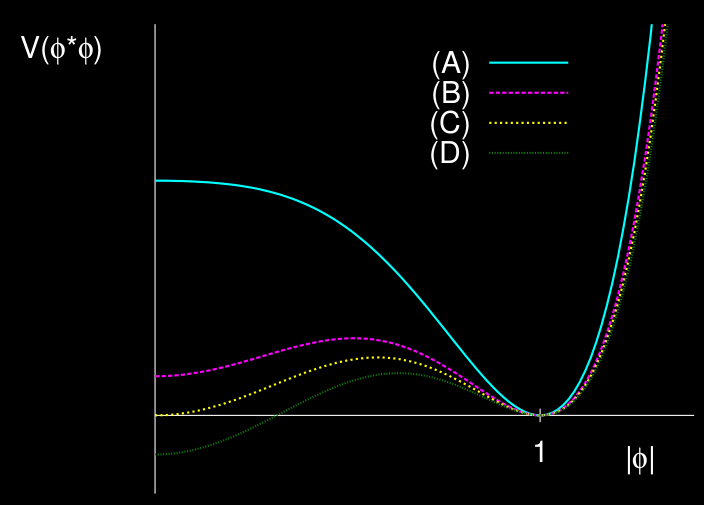
\includegraphics[scale=0.25]{evo_pot.png}
   %+ orientés désorientés ou juste tableau?
 \end{figure}
\end{frame}


%\item Univers primordial et théorie d'unification (particules)
%\item Atteinte du vide: brisure spontanée de symétrie
%image?



\subsection{Atteinte du vide}
\begin{frame}
\frametitle{Symétries en physique des particules}
\begin{block}{Brisure spontanée de symétrie}
Les lois de la nature peuvent posséder des symétries sans que l'état de vide (fondamental) le soit nécessairement
\begin{enumerate}
\item Boson: Goldstone, Higgs et les jauges
\item Glashow, Salam et Weinberg: $SU(2)xU(1)$ 
\end{enumerate}
\end{block}
Modèle standard permet les associations suivantes:
\begin{block}{Groupes de Lie pour les forces}
\begin{enumerate}
\item nucléaire faible: SU(2)
\item nucléaire forte: SU(3)
\item électromagnétique: U(1)
\end{enumerate}
\end{block}
\end{frame}

\begin{frame}
\frametitle{Ferroaimant de Heisenberg - Dipôles magnétiques sur réseau}
Invariance de H sous rotation - symétrie SO(2)\\
\begin{equation*}
H= -J\sum_{i}{\sum_{voisins j}{\vec{S}_i\cdot\vec{S}_j}}
\end{equation*} 
%État de plus basse énergie: dipôles alignés \\
 \begin{figure}[0.5\textwidth]
   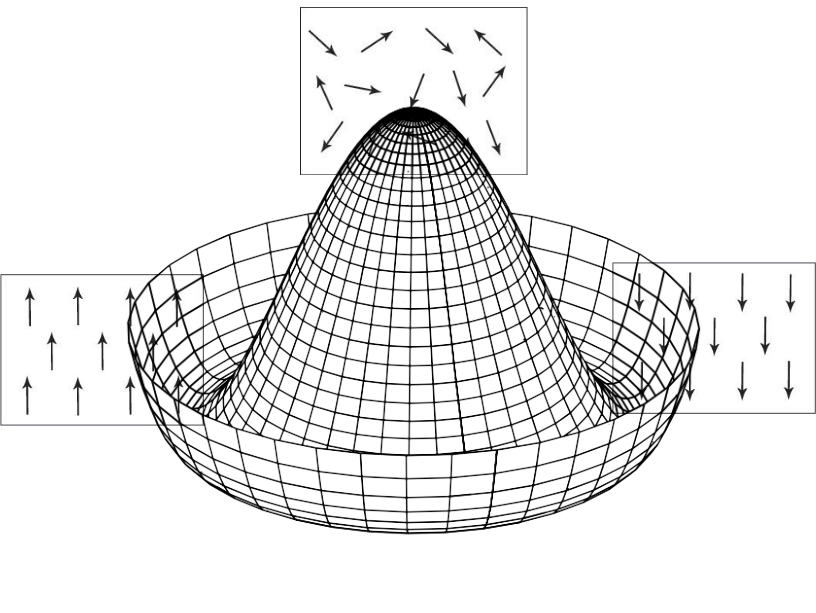
\includegraphics[scale=0.25]{potpot.png}

 \end{figure}

\end{frame}
%
%\begin{frame}
%    \begin{figure}[0.3\textwidth]
%   %\includegraphics[scale=0.25]{aimants_desorientes.jpg}
%    \end{figure}
%    Petit homme dans le réseau
%    
%Et bien plus encore: vortex pour expliquer les supra type I et II
% \end{frame} 

\begin{frame}
\begin{columns}[T]
\begin{column}[T]{.5\linewidth}
    \begin{enumerate}
    \item Température critique (Curie)
    \item Vides dégénérés, différant dans l'espace: défauts topologiques (solitons)
   % \item Rencontre: murs de domaine
    %\item $\rightarrow$ murs: liés aux solitons, défauts topologiques
    \end{enumerate}
    \end{column}
	\begin{column}[T]{.5\linewidth}
    \begin{figure}[0.3\textwidth]
    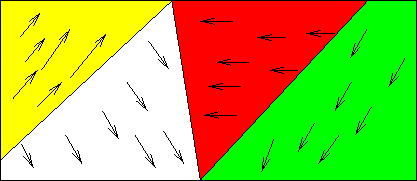
\includegraphics[scale=0.4]{murs.png}
    \end{figure}
 
	\end{column}
	
\end{columns}
\begin{figure}[0.3\textwidth]
    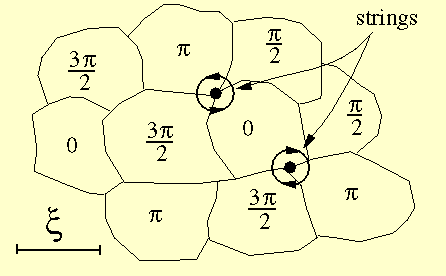
\includegraphics[scale=0.3]{string.png}
    \end{figure}
 

\end{frame}
\subsection{Symétrie et cosmologie}
%\begin{frame}
%
%\begin{columns}[T]
%    \begin{column}[T]{.5\linewidth}
%   \begin{figure}[0.3\textwidth]
%    %\includegraphics[scale=0.25]{pot_uni.jpg}
%    \end{figure}
%    \end{column}
%    \begin{column}[T]{.5\linewidth}
%    \begin{enumerate}
%    \item max: univers primordial (densité d'énergie)
%    \item min: notre état de l'univers?
%    \item transition, et apparition d'un vrai vide
%    \begin{enumerate}
%    \item possibilité de transition par effet tunnel
%    \item taux de désintégration; dégéneresence des faux vides
%    \end{enumerate}
%    \end{enumerate}
%        %figure Marie-Lou transition du potentiel
%    \end{column}
%  \end{columns}
%  \end{frame}
  
  \begin{frame}\frametitle{Fin de 1ère section}
  
  
  
\begin{columns}[T]
    \begin{column}[T]{.5\linewidth}
\textbf{Cosmologie - Retenez:}\\
Description de l'univers par un potentiel U
\begin{enumerate}
 \item Origine $\rightarrow$ max(U)
 \item État actuel \\ $\rightarrow$ métastable? \\ $\rightarrow$ symétrie brisée?
\end{enumerate}
    \end{column}
    \begin{column}[T]{.5\linewidth}
     \textbf{Outillage - Solitons:}\\
     $\rightarrow$ Symétrie brisée \\$\rightarrow$ Défauts topologiques \\$\rightarrow$ Solitons\\[0.5 cm]
     
     
     \textbf{Évolution de l'univers:}\\
     Solitons peuvent affecter le taux de transition vers un vrai vide
    \end{column}
  \end{columns}  
  
  
  
  
  
  
  
  
  
  
  
  
  
  
  

 
%    Symétries brisées spontanément: structure non triviale des vides
%    \textbf{Le taux de désintégration de l'univers peut être affecté par la présence de défauts topologiques. Est-ce que l'univers a connu une transition de phase avec brisure de symmétrie? Selon le modèle standard, possiblement. Alors, on attend des cordes cosmiques, monopôles magnétiques. Surtout, ces défauts topologiques pourrait affecter l'évolution actuelle de notre univers. C'est l'objet de notre étude.}
%    
  \end{frame}


%-----------------------------------------------------------------------------------------------------------------
\section{Solitons - Appareillage mathématique }

\subsection{Équation d'ondes et soliton}
%eq d'onde
\begin{frame}
\frametitle{Équation d'ondes}
Champ scalaire défini dans $\mathbb{R}^n$: $\phi(\vec{x},t)$\\
\begin{block}{Équation d'onde}
\begin{equation}
\frac{1}{c^2}\frac{\partial^2 \phi}{\partial t^2} - \nabla^2 \phi = \square \phi = 0 
\end{equation}
\textit{Deux propriétés étudiées dans les solutions $\phi$}
\begin{itemize}
\item Forme et vitesse de l'onde conservées\\
\item Deux ondes retrouvent asymptotiquement leur forme et vitesse\\
\end{itemize}
\end{block} 
\end{frame}

%potentiel de solitons
\begin{frame}
\begin{enumerate}
\item Équation d'onde: V=0
\end{enumerate}

\begin{block}{Potentiels différents - Équations du mouvements modifiées}
\begin{enumerate}

\item terme dispersif: $\square\phi +$ \boldmath $m^2 \phi $ \unboldmath  = 0 (Klein-Gordon)\\
\begin{enumerate}
\item onde plane: $k^2 \rightarrow k^2+m^2$

\end{enumerate}
\item terme non-linéaire: $\phi^3$ \\
\end{enumerate}
\end{block}
En s'éloignant de l'équation d'onde, les deux propriétés peuvent être conservées: ondes solitaires et solitons 

\end{frame}

%photo Russell pour le plaisir
\begin{frame}
Sur sa monture, John Russell poursuit sa destinée, vers l'onde solitaire!
\begin{columns}[T]
    \begin{column}[T]{.5\linewidth}
   \begin{figure}[0.3\textwidth]
 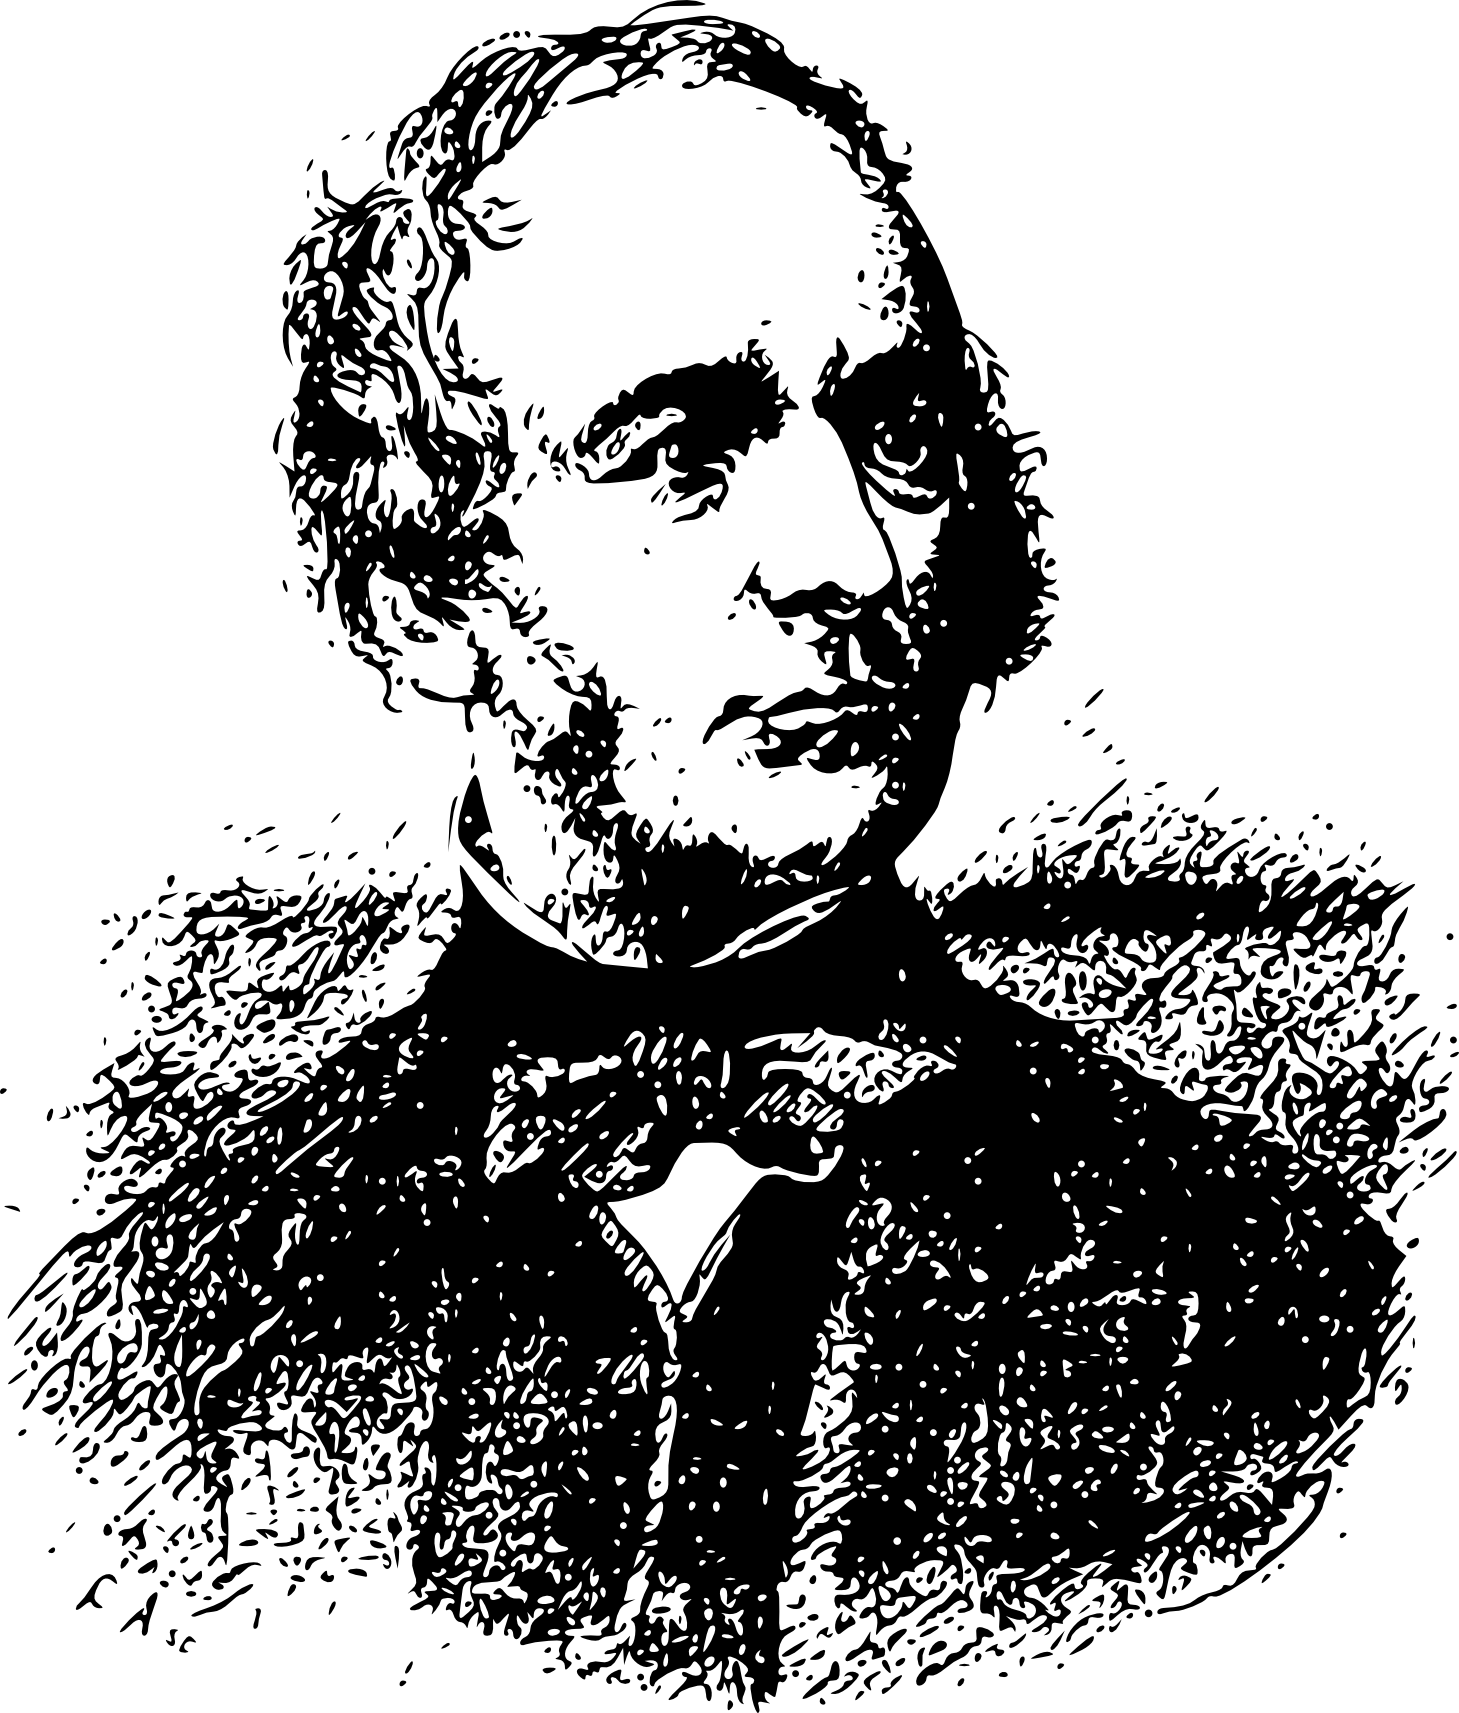
\includegraphics[scale=0.25]{russell.png}
    \end{figure}
    \end{column}
    \begin{column}[T]{.5\linewidth}
    \begin{figure}[0.3\textwidth]
   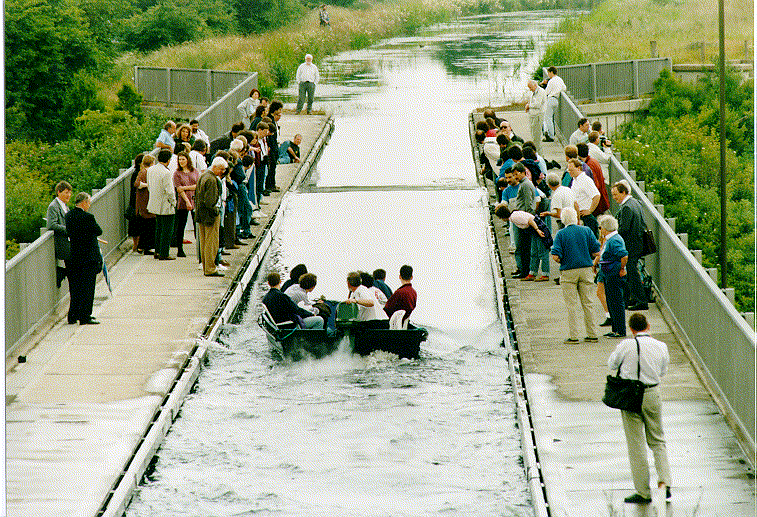
\includegraphics[scale=0.2]{soliton1b.png}
    \end{figure}
    \end{column}
  \end{columns}
\end{frame}


\begin{frame}\frametitle{Description d'un soliton topologique}

	\begin{enumerate}
	\item Densité d'énergie d'un soliton: 
	\begin{enumerate}
	\item Localisée dans l'espace (finitude)
	\item Conservée et non-nulle (solution non-dissipative, exigence topologique)
	\end{enumerate}

				\begin{align*}
	E[\phi] = \int{dxdt (\mathcal{H}[\phi])} = \int{dxdt [\frac{1}{2} (\partial_x \phi)^2 + V(\phi)]}
	\end{align*}
	\item Énergie finie:
	\begin{enumerate}
	\item  $\lim\limits_{x \to \pm\infty}\partial_x \mathcal{H} =0$
	\item  $\lim\limits_{x \to \pm\infty} \phi[x] = g^{(i)}$ où les $g^{(i)}$ sont les min. de V	
	\end{enumerate}	
	\item Structure des vides non triviale
	\end{enumerate}

		\end{frame}
	\begin{frame}\frametitle{En image}

	\begin{figure}[0.3\textwidth]
   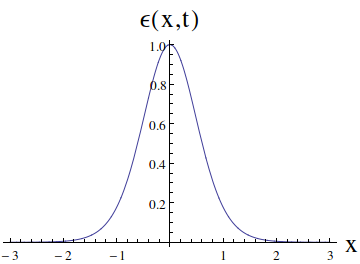
\includegraphics[scale=0.5]{densite.png}
    \end{figure}
	

\end{frame}


\subsection{Formalisme Lagrangien}
\begin{frame}

\frametitle{Formalisme Lagrangien}

\begin{block}{Notation covariante}

\begin{enumerate}
\item $x_0 = ct \hspace{1 cm} x_{1,2,3} = x,y,z$
\item $x^\mu = (x_0,\vec{x})$ et $x^\mu = (x_0,-\vec{x})$
\item Métrique: $x^\mu = g^{\nu\mu} x_\nu$
\item Minkowski: $\eta^{\nu\mu} \rightarrow diag(1,-1,-1,-1)$
%\item indices répétés: $v_a \cdot v_a = \sum_{i=0}^{3}x_i^2$ (produit scalaire)
\end{enumerate}

\end{block}
\begin{align*}
\partial^\mu =& (\frac{1}{c} \partial_t, -\nabla) \\
\partial_\mu \partial^\mu =& \frac{1}{c^2} \partial_t^2- \nabla^2
\end{align*}
\end{frame}

\begin{frame}
\begin{enumerate}
\item \textit{Action}: $S[\phi] = \int{dt (L[\phi])}  =  \int{dx_\mu (\mathcal{L}[\phi])}$
\begin{enumerate}
\item Principe d'Hamilton: $\phi_0$ | action minimisée \\
\item Premier ordre nul pour un minimum d'action \\
\end{enumerate}
\item  $\mathcal{L}[\phi] = \frac{1}{2} \partial_\mu \phi (\partial^\mu \phi)^* -V$
\item \textit{Euler-Lagrange:} $\partial_\mu \left(\frac{\mathcal{L}}{\partial(\partial_\mu\phi)}\right) = \frac{\partial\mathcal{L}}{\partial\phi}$
\end{enumerate}
\begin{exampleblock}{Équation d'ondes - V=0}
Par Euler-Lagrange:
\begin{align*}
 \partial_\mu(\frac{\partial_a\phi (\partial^a\phi)^* }{\partial_\mu \phi}) = 0 \\
\partial_\mu (\partial^\mu \phi)^*  = 0 \\
 \square \phi = 0 \\
\end{align*}

\end{exampleblock}

\end{frame}

\subsection{Kink}
\begin{frame}
\frametitle{Kink: cas de figure typique}
\begin{block}{Potentiel d'ordre 4}

    \begin{equation*}
    V(\phi) = \frac{\lambda}{4}(|\phi|^2 -\frac{m^2}{\lambda})^2
    \end{equation*}
    \begin{figure}
     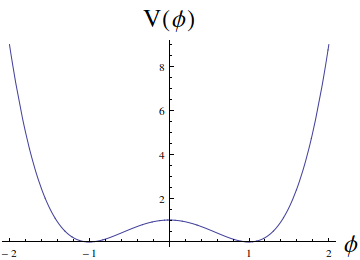
\includegraphics[scale=0.5]{pot_z2.png}
    \end{figure}


\end{block}
%$\mathcal{L} = \frac{1}{2}(\partial_x \phi)^2 - V $ \\
%$\rightarrow \phi'' = \lambda \phi^3 - m^2 \phi$ \\
\end{frame}
\begin{frame} \frametitle{Analogie mécanique classique}
\begin{equation*}
\mathcal{H}[\phi] = \frac{1}{2} \partial_\mu \phi (\partial_\mu \phi)^* +V
\end{equation*}
\begin{columns}[T]
    \begin{column}[T]{.55\linewidth}
    Champ
    \begin{enumerate}
    \item $\mathcal{H} =  \cancelto{}{\frac{1}{2}  (\partial_t \phi)^2} +  \frac{1}{2}  (\partial_x \phi)^2 +V(\phi) $
%    \item $\frac{\partial^2\phi}{\partial_x^2} = \frac{\partial V}{\partial\phi}$
    \item $E_\phi = \int{dx\left[\frac{1}{2}  (\partial_x \phi)^2 +V(\phi) \right]}$
    \end{enumerate}
    \end{column}
    \begin{column}[T]{.45\linewidth}
	Particule
    \begin{enumerate}
    \item $L =   \frac{1}{2}  \dot{q}^2 -U(q)$
%    \item $\frac{\partial^2\phi}{\partial_x^2} = -\frac{\partial U}{\partial\phi}$
    \item $S_q = \int{dt[\frac{1}{2}  \dot{q}^2 -U(q)] }$
    \end{enumerate}
    \end{column}
  \end{columns}
  
 
    $E_\phi$ finie $\leftrightarrow S_q$ finie $\rightarrow E_q = 0$\\
 On étudie alors: -V

  
\end{frame}

\begin{frame}
\begin{figure}
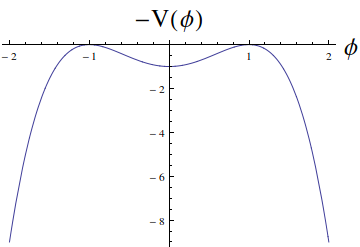
\includegraphics[scale=0.5]{pot_inv.png}
\end{figure}
Solution privilégiée: D'un max à l'autre
\end{frame}

\begin{frame}
Récapitulons:
\begin{enumerate}
\item 1+1 dimensions, mais solution statique
\item Potentiel V d'ordre 4 
\item Équations d'Euler-Lagrange $\rightarrow$ Équations du mouvement: 
\begin{enumerate}
\item $\rightarrow \phi'' = \lambda \phi^3 - m^2 \phi$ (équation statique)
\item solution: kink
\end{enumerate}
\end{enumerate}
\end{frame}

\begin{frame}\frametitle{Kink}
\begin{align*}
\phi(x) = \frac{m}{\sqrt{\lambda}}tanh\left[\frac{m}{\sqrt{2}}(x-x_0)\right]
\end{align*}
\begin{figure}
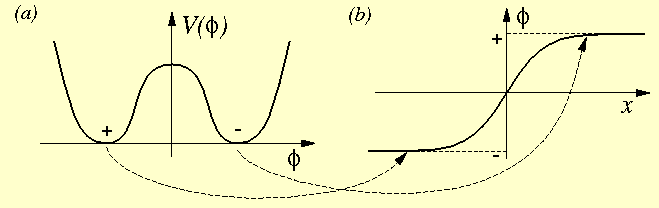
\includegraphics[scale=0.4]{soli_def.png}
\end{figure}


\begin{enumerate}
\item Défaut topologique et déformations continues
\item Mur de domaine (symétrie discrète brisée, 1 dimension)
\item En plusieurs dimensions, cordes cosmiques, monopôles
\end{enumerate}
\end{frame}

\begin{frame}\frametitle{Retour - Cosmologie et solitons}
\begin{enumerate}
\item Cosmologie et brisure de symétrie dans la nature (MS, ferroaimant)
\item Évidences expérimentales pour une brisure de symétrie
\end{enumerate}
\begin{enumerate}
\item Expression des brisures de symétrie: défauts topologiques, solitons
\item Structure non triviale des vides: $solitons \leftrightarrow univers$
\end{enumerate}



\end{frame}

\begin{frame}
Taux de désintégration: effet tunnel quantique
\begin{figure}[0.5\textwidth]
   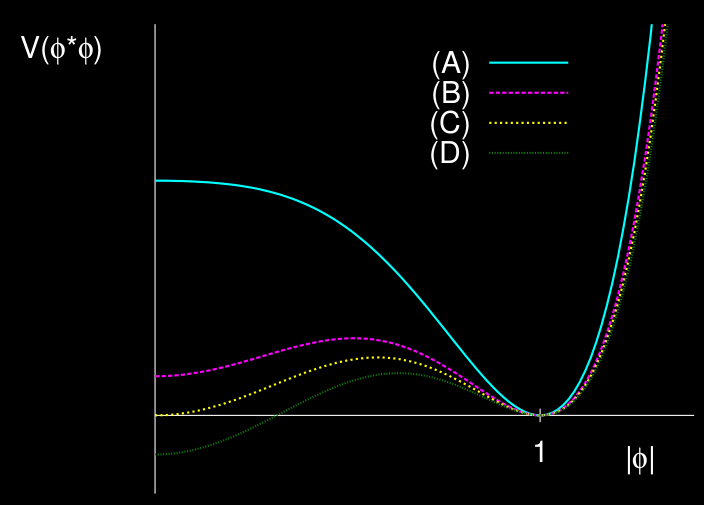
\includegraphics[scale=0.25]{evo_pot.png}
   %+ orientés désorientés ou juste tableau?
 \end{figure}
Potentiel inversé: recherche du chemin de moindre action (Euclidienne) $\rightarrow$ bounce \\
Intégrale de chemin: $ \tau/V \approx e^{-So/\hbar}$ \\
Fluctuation d'un soliton: autre source de désintégration!!!\\
\end{frame}




%-----------------------------------------------------------------------------------------------------------------

\section{Quotidien en cosmologie théorique des particules}
\begin{frame}
%potentiel avec lequel on travaille
\begin{block}{Potentiel à deux champs $\phi(x,t)$ et $\psi(x,t)$}
\begin{equation*}
V(\phi,\psi)=(\psi^2-\delta_1)(\psi^2-1)^2+\frac{\alpha}{\psi^2+\gamma}[(\phi^2-1)^2 - \frac{\delta_2}{4}(\phi-2)(\phi+1)^2] 
\end{equation*}

\end{block}
\begin{columns}[T]
    \begin{column}[T]{.5\linewidth}
  
\begin{enumerate}
\item 1+1 dimensions (x,t) mais on cherche une solution statique
\item Beaucoup de paramètres: $\alpha, \gamma, \delta_1, \delta_2$
\item Les champs sont couplés
\end{enumerate}  
    \end{column}
    \begin{column}[T]{.5\linewidth}
    \begin{figure}[0.3\textwidth]
    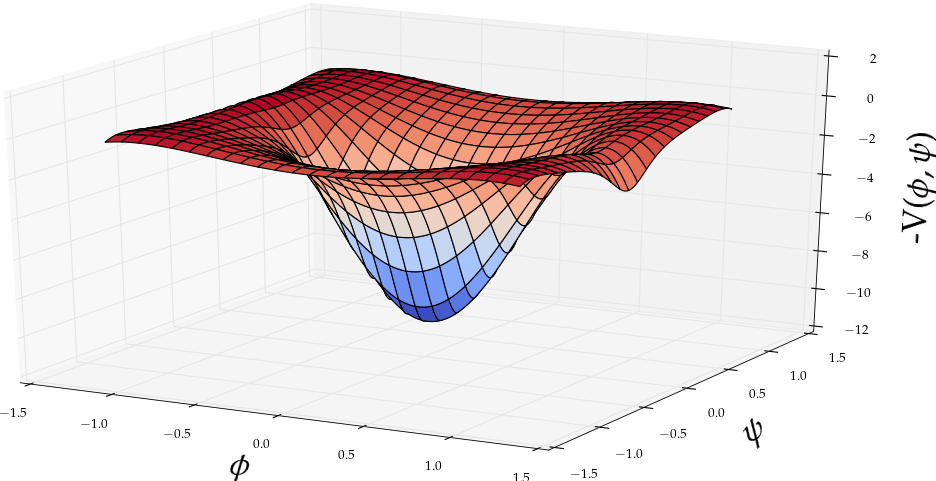
\includegraphics[scale=0.2]{Capture-2.png}
    \end{figure}
    \end{column}
  \end{columns}
\end{frame}

\begin{frame}
Pourquoi bâtir un potentiel comme ça en premier lieu?!?!\\
\begin{figure}[0.3\textwidth]
    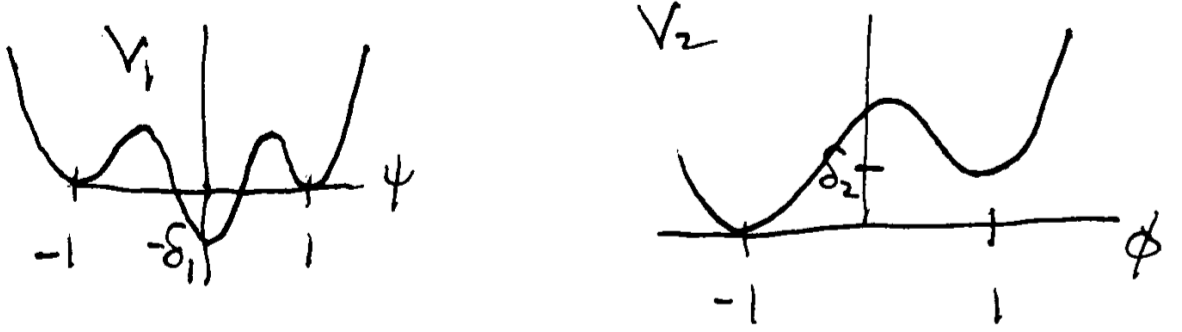
\includegraphics[scale=0.25]{psi_phi.png}
    \end{figure}
\begin{columns}[T]
    \begin{column}[T]{.5\linewidth}
    \begin{enumerate}
    \item $\delta_1 \rightarrow$ contrôle du minima central
    \item Potentiel d'ordre 6, CLASSIQUE! 
    \end{enumerate}
   
    \end{column}
    \begin{column}[T]{.5\linewidth}
    \begin{enumerate}
    \item    $\delta_2 \rightarrow$ Contrôle de la séparation entre minimum sur l'axe $\phi$
    \end{enumerate}

    \end{column}
  \end{columns}
  
 $\alpha$: Importance du 2ème terme \\
 $\gamma$: Importance du couplage \\
\end{frame}

\begin{frame}\frametitle{À venir...}
\begin{enumerate}
\item Trouver des solutions aux équations de mouvements (contraintes à $\lim\limits_{x \to \pm\infty}$)
\end{enumerate}
\begin{figure}[0.3\textwidth]
     %%\includegraphics[scale=0.25]{potphi.png}
    \end{figure}
\begin{enumerate}
    \item Tester la stabilité de la solution
    \end{enumerate} 
    
\begin{figure}[0.3\textwidth]
     %%\includegraphics[scale=0.25]{potphi.png}
    \end{figure}
    
\begin{enumerate}
   \item Trouver une borne maximale sur l'action $\rightarrow$ borne minimale sur $\tau$
   \end{enumerate}   
    
\end{frame}

\end{document}